\chapter{Practice}
The practical part of this thesis can be found in this chapter.
It gives information about the Datasets and feature extraction of its data used for training the Neural Network architectures.
Further here is the evaluation of the Neural Network models and
the evolution process of the individual approaches used for speech command classification.
Also the implementation of the Key Word Spotting system and some Game Design ideas of possible applications with speech commands are given.


% dataset
% --
% dataset

\section{Dataset}
This section discusses the used datasets as input to the machine learning architectures for speech command classification.
The dataset details and properties of the sound files are presented.
Some sound examples and their feature representation of the datasets is shown.
Further the quality and diversity of recorded samples is mentioned.

\begin{table}[ht!]
\begin{center}
\caption{Dataset reference with feature group extraction.}
\begin{tabular}{ M{2cm} M{8cm} }
\toprule
%\multicolumn{4}{c}{\textbf{Feature Groups}} & \multicolumn{2}{c}{\textbf{Accuracy}} \\
\textbf{Abbreviation} & \textbf{Meaning}\\
\midrule
c[0-1] & use of cepstral features, 0 is false and 1 is true\\ 
d[0-1] & use of delta features\\ 
dd[0-1] & use of double delta features\\ 
e[0-1] & use of energy features\\
norm & features are normalized over frames\\
\bottomrule
\label{tab:feature_groups}
\end{tabular}
\end{center}
\end{table}
\FloatBarrier
\noindent

% --
% Speech Commands dataset

\subsection{Speech Commands Dataset}
The Speech Command Dataset \cite{warden2018} is a very diverse dataset consisting of over thousands of different speakers. This dataset is by any means no clean dataset recorded by professionals, if anything it is the opposite. 
The audio files are not normalized, there are samples with inconsistent sample numbers and some examples are prone with too much noise or even noise only.
And its still great, because there is no need for a perfect dataset and one can be happy that there exists one with this amount of diversity and free of access.
In fact maybe its even better to have an unclean dataset, so that invariances against noise are learnt and do not have be added by hand.
Some examples in raw audio format is shown in \rfig{dataset_wav_grid_c30}.
\begin{figure}[!ht]
  \centering
    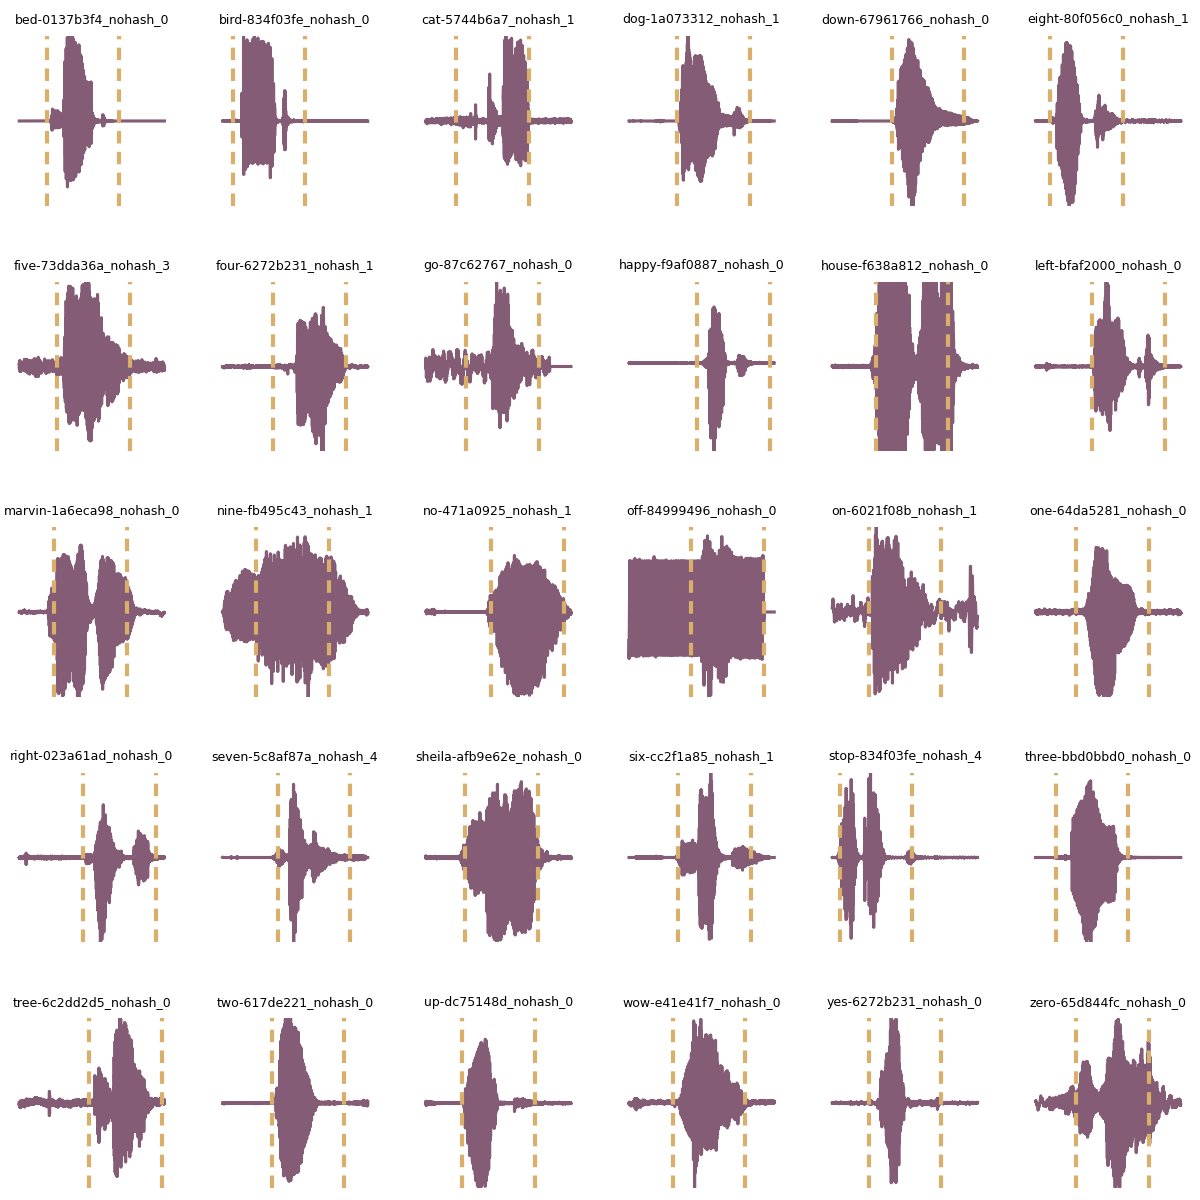
\includegraphics[width=0.65\textwidth]{./4_practice/figs/dataset_wav_grid_c30}
  \caption{Random samples from the Speech Command Dataset, one per class. Pre-processed and normalized raw audio data.}
  \label{fig:dataset_wav_grid_c30}
\end{figure}
\FloatBarrier
\noindent

\subsubsection{Extraction for Training}
The Speech Commands Dataset is extracted before it is used for training. 
To reduce computations in the evaluation process of Neural Networks, it was important to reduce the number of classes and examples per class to an suitable number.
In the Evaluation of Neural Networks the datasets the references in \rtab{dataset_refs} are used

\begin{table}[ht!]
\begin{center}
\caption{Dataset references with label restrictions in number of labels and labels itself.}
\begin{tabular}{ M{2cm}  M{2cm}  M{5cm} }
\toprule
%\multicolumn{4}{c}{\textbf{Feature Groups}} & \multicolumn{2}{c}{\textbf{Accuracy}} \\
\textbf{Reference name} & \textbf{Number of examples per label} & \textbf{Selected Labels}\\
\midrule
n500-c5 & 500 & left, right, up, down, go\\
n500-c10 & 500 & yes, no, left, go, down, off, right, stop, up, on\\
n500-c30 & 500 & \enquote{all}\\
\bottomrule
\label{tab:dataset_refs}
\end{tabular}
\end{center}
\end{table}
\FloatBarrier
\noindent

% --
% my dataset

\subsection{My own Dataset}
The author of this thesis recorded some speech command samples by himself and used it as own test set in evaluating trained models in the machine learning part. No self recorded files are used within the training set, so that it can be shown that unseen voice characteristics are classified correctly.
All examples of my own dataset are illustrated in \rfig{dataset_wav_grid_my} in raw audio format.

\begin{figure}[!ht]
  \centering
    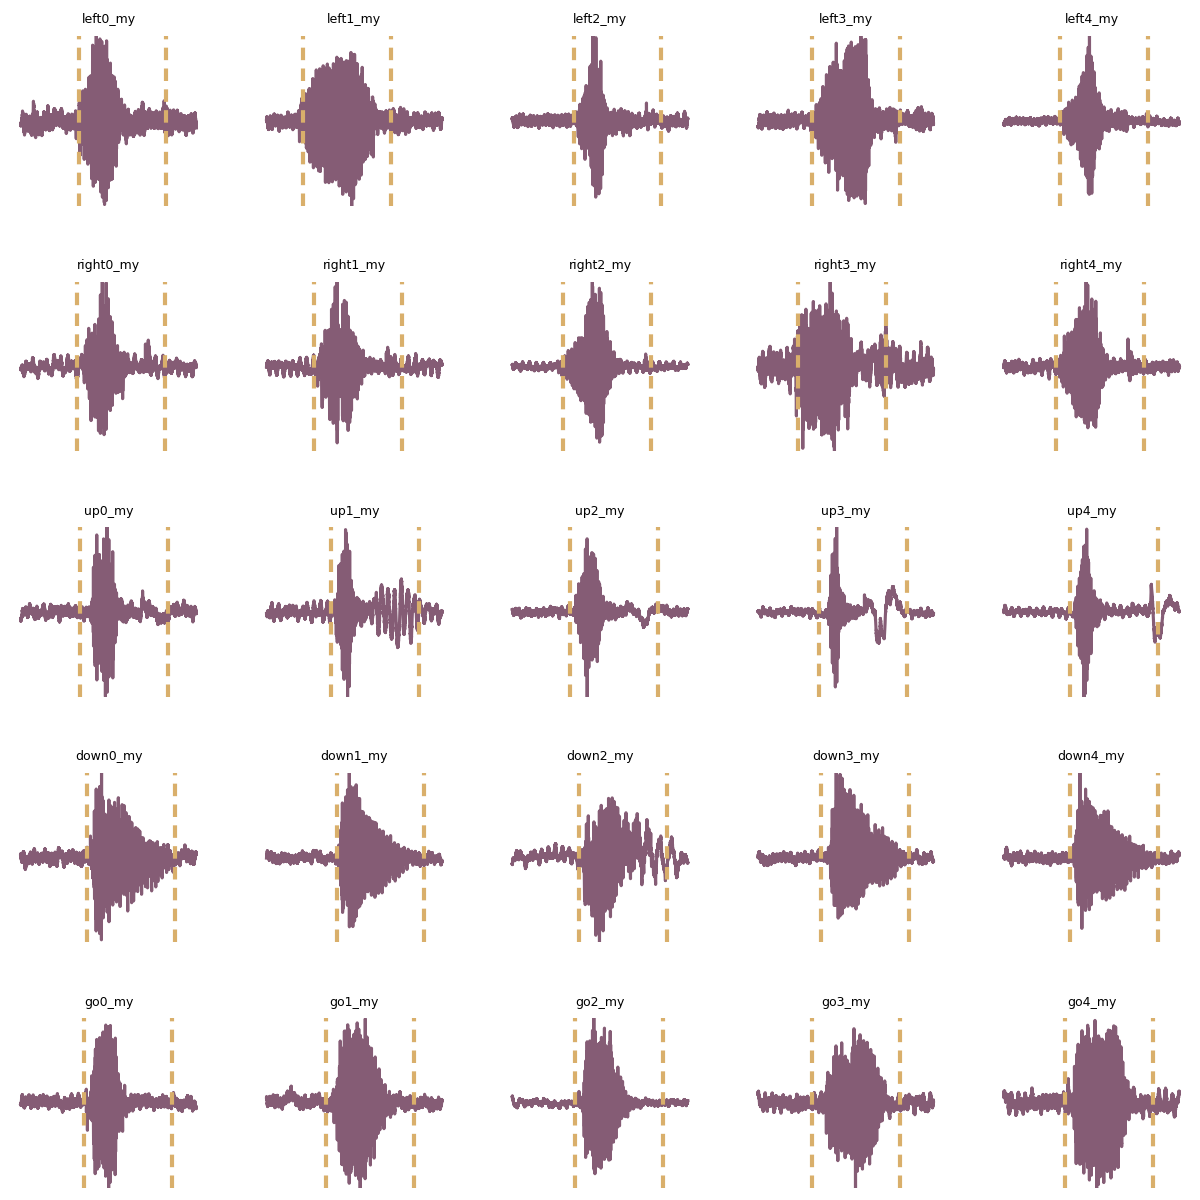
\includegraphics[width=0.65\textwidth]{./4_practice/figs/dataset_wav_grid_my}
  \caption{My wav grid}
  \label{fig:dataset_wav_grid_my}
\end{figure}
\FloatBarrier
\noindent

% machine learning
\section{Machine Learning Evaluation}\label{sec:ml}
In this section, the machine learning evaluation of the mentioned Neural Network Architectures, denoted here also simply as models, are presented.
The training details are listed to give the reader an overview of the selected parameters for training, it should also give a shorten reference, so that not all parameters must be listed in the plots. 
The training and evaluation consists of following evaluation tasks:
\begin{enumerate}
  \item Feature Selection
  \item Adversarial Training
\end{enumerate}

% --
% ml details

\subsection{Training Details}
We can separate the training details into following parameters to select from:
\begin{enumerate}
  \item Features extraction parameters
  \item Dataset parameters
  \item Feature selection
  \item Transfer Learning parameters
  \item Machine Learning parameters
\end{enumerate}
The feature extraction parameters simply give information about how features are extracted, e.g. this includes the hop size, frame size, filter bands of the MFCC, etc.
The dataset parameters are the information of which labels and how many examples per labels are used
Also they consist of the feature selection, so that the extracted dataset only consists of MFCC data. 
The Abbreviation regarding dataset parameters and feature selection were already listed in \rtab{dataset_abbr}.
%The feature selection is the information about what input feature groups are used in the training, e.g. use cepstral coefficients only, or add delta and energy features, their references are shown in \rtab{dataset_feature_groups}.
The Transfer Learning parameters are pre-trained weights for the actual neural network architecture to be trained.
This could be only the first convolutional layers or entire networks but here all convolutional layers from an adversarial training are considered. 
The Abbreviations for training parameters can be specified as listed in \rtab{ml_details_adv}
\begin{table}[ht!]
\begin{center}
\caption{Adversarial Training abbreviations.}
\begin{tabular}{ M{2cm}  M{5cm} }
\toprule
%\multicolumn{4}{c}{\textbf{Feature Groups}} & \multicolumn{2}{c}{\textbf{Accuracy}} \\
\textbf{Abbreviations} & \textbf{Meaning}\\
\midrule
dec & use of decoder weights\\
enc & use of encoder weights\\
itl[0-9]+ & iterations per label, e.g. itl500 for 500 iterations\\
\bottomrule
\label{tab:ml_details_adv}
\end{tabular}
\end{center}
\end{table}
\FloatBarrier
\noindent


The Machine Learning parameters are classically training parameters such as learning rate, number of epochs, etc.
Their selection and references are listed in \rtab{ml_details_train_params}

\begin{table}[ht!]
\begin{center}
\caption{All training parameters used within this thesis and their abbreviations.}
\begin{tabular}{ M{2cm}  M{5cm} }
\toprule
%\multicolumn{4}{c}{\textbf{Feature Groups}} & \multicolumn{2}{c}{\textbf{Accuracy}} \\
\textbf{Abbreviations} & \textbf{Meaning}\\
\midrule
it[0-9]+ & Number of epochs (or iterations)\\
bs[0-9]+ & Batch size, e.g. bs32 is a batch size of 32 examples\\
lr[0-9.]+ & Learning rate, e.g. lr0.0001\\
mo[0-9.]+ & Momentum, e.g. mo0.5\\
\bottomrule
\label{tab:ml_details_train_params}
\end{tabular}
\end{center}
\end{table}
\FloatBarrier
\noindent


% --
% feature selection

\subsection{Feature Selection}
The first important Question, when using Neural Networks, is what features are used as inputs.
In the theory section about MFCCs \rsec{t_mfcc}, it was shown how raw audio files can be extracted to MFCCs and what enhancements can be done.
These enhancements (deltas and energy features) are formed in groups for evaluation to see the impact on the choice and hopefully to reduce the input feature size to a minimum.
%Now that the Neural Network Architectures are described in \rsec{nn_arch} and basic knowledge about MFCCs is given in \rsec{features} it is important to evaluate the impact of the selection of certain MFCC feature constellations to the accuracy of the Test sets.
Beside it is good to get a general overview on what accuracies can be expected from different Neural Network Architectures.
The evaluation is done on 5 classes and 30 classes with different training parameters to observe the impact on a easy and a very hard classification task.
In detail it is shown how models are trained with features consisting of following MFCC groups:
\begin{enumerate}
    \item Cepstral Coefficients (usual MFCCs)
    \item Deltas (frame difference of MFCCs)
    \item Double Deltas (frame difference of Deltas)
    \item Energy Vector (added to each of the upper features)
\end{enumerate}
Another crucial point is to evaluate whether a frame based normalization of these features hurt the training and the accuracy of the models.
Therefore additional columns are presented in the following tables marked with \enquote{norm}.
Note that all these experiments have been done with n-500 a number of 500 examples per class, so that computations are minimized but still enough data is drawn.

\subsubsection{Feature Selection on Conv Encoder}
The feature selection evaluation on the conv-encoder-fc1 architecture with 5 labels is listed in \rtab{fs_fc1_it500_c5}.
% \begin{table}[ht!]
\begin{center}
\caption{Feature Selection ml it500 c5 features fc1}
\begin{tabular}{ M{1cm}  M{1cm}  M{1cm}  M{1cm}  M{1.5cm}  M{1.5cm}  M{1.5cm}  M{1.5cm} }
\toprule
\multicolumn{4}{c}{\textbf{Feature Groups}} & \multicolumn{2}{c}{\textbf{Accuracy}} \\
\textbf{c} & \textbf{d} & \textbf{dd} & \textbf{e} & \textbf{acc test} & \textbf{acc my} & \textbf{acc test norm} & \textbf{acc my norm} \\
\midrule
0 & 0 & 1 & 0 & 86.67 & 80.00 & 68.33 & 73.33 \\
0 & 0 & 1 & 1 & 85.00 & 86.67 & 67.67 & 73.33 \\
0 & 1 & 0 & 0 & 92.67 & 100.00 & 75.67 & 80.00 \\
0 & 1 & 0 & 1 & 90.67 & 90.00 & 82.00 & 73.33 \\
0 & 1 & 1 & 0 & 91.00 & 93.33 & 76.67 & 70.00 \\
0 & 1 & 1 & 1 & 89.33 & 100.00 & 78.67 & 80.00 \\
1 & 0 & 0 & 0 & 16.67 & 16.67 & 88.33 & 86.67 \\
1 & 0 & 0 & 1 & 33.33 & 33.33 & 86.33 & 80.00 \\
1 & 0 & 1 & 0 & 91.00 & 90.00 & 87.00 & 80.00 \\
1 & 0 & 1 & 1 & 82.67 & 86.67 & 86.67 & 90.00 \\
1 & 1 & 0 & 0 & 91.67 & 76.67 & 88.33 & 90.00 \\
1 & 1 & 0 & 1 & 90.00 & 80.00 & 89.33 & 93.33 \\
1 & 1 & 1 & 0 & 89.00 & 76.67 & 89.33 & 90.00 \\
1 & 1 & 1 & 1 & 88.00 & 90.00 & 89.00 & 86.67 \\
\bottomrule
\end{tabular}
\end{center}
\label{tab:ml_it500_c5_features_fc1}
\end{table}
\FloatBarrier
\noindent


% \begin{table}[ht!]
\begin{center}
\caption{Feature Selection ml it1000 c30 features fc1}
\begin{tabular}{ M{1cm}  M{1cm}  M{1cm}  M{1cm}  M{1.5cm}  M{1.5cm} }
\toprule
\multicolumn{4}{c}{\textbf{Feature Groups}} & \multicolumn{2}{c}{\textbf{Accuracy}} \\
\textbf{c} & \textbf{d} & \textbf{dd} & \textbf{e} & \textbf{acc test} & \textbf{acc test norm} \\
\midrule
0 & 0 & 1 & 0 & 52.97 & 33.10 \\
0 & 0 & 1 & 1 & 56.65 & 27.94 \\
0 & 1 & 0 & 0 & 63.55 & 39.68 \\
0 & 1 & 0 & 1 & 74.52 & 48.65 \\
0 & 1 & 1 & 0 & 71.03 & 39.35 \\
0 & 1 & 1 & 1 & 73.94 & 46.39 \\
1 & 0 & 0 & 0 & 47.23 & 58.19 \\
1 & 0 & 0 & 1 & 45.35 & 57.81 \\
1 & 0 & 1 & 0 & 60.45 & 47.55 \\
1 & 0 & 1 & 1 & 59.48 & 51.61 \\
1 & 1 & 0 & 0 & 58.77 & 55.10 \\
1 & 1 & 0 & 1 & 6.45 & 47.81 \\
1 & 1 & 1 & 0 & 65.81 & 60.39 \\
1 & 1 & 1 & 1 & 62.06 & 51.55 \\
\bottomrule
\end{tabular}
\end{center}
\label{tab:ml_it1000_c30_features_fc1}
\end{table}
\FloatBarrier
\noindent


% \begin{table}[ht!]
\begin{center}
\caption{Feature Selection ml it2000 c30 features fc3}
\begin{tabular}{ M{1cm}  M{1cm}  M{1cm}  M{1cm}  M{1.5cm}  M{1.5cm} }
\toprule
\multicolumn{4}{c}{\textbf{Feature Groups}} & \multicolumn{2}{c}{\textbf{Accuracy}} \\
\textbf{c} & \textbf{d} & \textbf{dd} & \textbf{e} & \textbf{acc test} & \textbf{acc test norm} \\
\midrule
0 & 0 & 1 & 0 & 49.03 & 33.74 \\
0 & 0 & 1 & 1 & 66.90 & 34.84 \\
0 & 1 & 0 & 0 & 77.10 & 55.55 \\
0 & 1 & 0 & 1 & 78.65 & 56.52 \\
0 & 1 & 1 & 0 & 74.97 & 50.26 \\
0 & 1 & 1 & 1 & 73.94 & 59.61 \\
1 & 0 & 0 & 0 & 76.52 & 64.26 \\
1 & 0 & 0 & 1 & 73.87 & 59.16 \\
1 & 0 & 1 & 0 & 78.58 & 63.03 \\
1 & 0 & 1 & 1 & 73.48 & 59.03 \\
1 & 1 & 0 & 0 & 79.10 & 66.13 \\
1 & 1 & 0 & 1 & 80.39 & 60.77 \\
1 & 1 & 1 & 0 & 76.97 & 64.71 \\
1 & 1 & 1 & 1 & 75.94 & 65.55 \\
\bottomrule
\end{tabular}
\end{center}
\label{tab:ml_it2000_c30_features_fc3}
\end{table}
\FloatBarrier
\noindent


\begin{table}[ht!]
\begin{center}
\caption{Feature Selection on arch: conv-encoder-fc1 with dataset: L5-n500 and training params: it500-bs32-lr0.0001-mo0.5}
\begin{tabular}{ M{1cm}  M{1cm}  M{1cm}  M{1cm}  M{1.5cm}  M{1.5cm}  M{1.5cm}  M{1.5cm} }
\toprule
\multicolumn{4}{c}{\textbf{Feature Groups}} & \multicolumn{2}{c}{\textbf{Accuracy}} \\
\textbf{c} & \textbf{d} & \textbf{dd} & \textbf{e} & \textbf{acc test} & \textbf{acc my} & \textbf{acc test norm} & \textbf{acc my norm} \\
\midrule
0 & 0 & 1 & 0 & 86.67 & 80.00 & 68.33 & 73.33 \\
0 & 0 & 1 & 1 & 85.00 & 86.67 & 67.67 & 73.33 \\
0 & 1 & 0 & 0 & 92.67 & 100.00 & 75.67 & 80.00 \\
0 & 1 & 0 & 1 & 90.67 & 90.00 & 82.00 & 73.33 \\
0 & 1 & 1 & 0 & 91.00 & 93.33 & 76.67 & 70.00 \\
0 & 1 & 1 & 1 & 89.33 & 100.00 & 78.67 & 80.00 \\
1 & 0 & 0 & 0 & 16.67 & 16.67 & 88.33 & 86.67 \\
1 & 0 & 0 & 1 & 33.33 & 33.33 & 86.33 & 80.00 \\
1 & 0 & 1 & 0 & 91.00 & 90.00 & 87.00 & 80.00 \\
1 & 0 & 1 & 1 & 82.67 & 86.67 & 86.67 & 90.00 \\
1 & 1 & 0 & 0 & 91.67 & 76.67 & 88.33 & 90.00 \\
1 & 1 & 0 & 1 & 90.00 & 80.00 & 89.33 & 93.33 \\
1 & 1 & 1 & 0 & 89.00 & 76.67 & 89.33 & 90.00 \\
1 & 1 & 1 & 1 & 88.00 & 90.00 & 89.00 & 86.67 \\
\bottomrule
\label{tab:fs_fc1_it500_c5}
\end{tabular}
\end{center}
\end{table}
\FloatBarrier
\noindent


\begin{table}[ht!]
\begin{center}
\caption{Feature Selection on arch: conv-encoder-fc1 with dataset: L30-n500 and training params: it1000-bs128-lr0.0001-mo0.5}
\begin{tabular}{ M{1cm}  M{1cm}  M{1cm}  M{1cm}  M{1.5cm}  M{1.5cm} }
\toprule
\multicolumn{4}{c}{\textbf{Feature Groups}} & \multicolumn{2}{c}{\textbf{Accuracy}} \\
\textbf{c} & \textbf{d} & \textbf{dd} & \textbf{e} & \textbf{acc test} & \textbf{acc test norm} \\
\midrule
0 & 0 & 1 & 0 & 52.97 & 33.10 \\
0 & 0 & 1 & 1 & 56.65 & 27.94 \\
0 & 1 & 0 & 0 & 63.55 & 39.68 \\
0 & 1 & 0 & 1 & 74.52 & 48.65 \\
0 & 1 & 1 & 0 & 71.03 & 39.35 \\
0 & 1 & 1 & 1 & 73.94 & 46.39 \\
1 & 0 & 0 & 0 & 47.23 & 58.19 \\
1 & 0 & 0 & 1 & 45.35 & 57.81 \\
1 & 0 & 1 & 0 & 60.45 & 47.55 \\
1 & 0 & 1 & 1 & 59.48 & 51.61 \\
1 & 1 & 0 & 0 & 58.77 & 55.10 \\
1 & 1 & 0 & 1 & 6.45 & 47.81 \\
1 & 1 & 1 & 0 & 65.81 & 60.39 \\
1 & 1 & 1 & 1 & 62.06 & 51.55 \\
\bottomrule
\label{tab:fs_fc1_it1000_c30}
\end{tabular}
\end{center}
\end{table}
\FloatBarrier
\noindent


\begin{table}[ht!]
\begin{center}
\caption{Feature Selection ml it2000 c30 features fc3}
\begin{tabular}{ M{1cm}  M{1cm}  M{1cm}  M{1cm}  M{1.5cm}  M{1.5cm} }
\toprule
\multicolumn{4}{c}{\textbf{Feature Groups}} & \multicolumn{2}{c}{\textbf{Accuracy}} \\
\textbf{c} & \textbf{d} & \textbf{dd} & \textbf{e} & \textbf{acc test} & \textbf{acc test norm} \\
\midrule
0 & 0 & 1 & 0 & 49.03 & 33.74 \\
0 & 0 & 1 & 1 & 66.90 & 34.84 \\
0 & 1 & 0 & 0 & 77.10 & 55.55 \\
0 & 1 & 0 & 1 & 78.65 & 56.52 \\
0 & 1 & 1 & 0 & 74.97 & 50.26 \\
0 & 1 & 1 & 1 & 73.94 & 59.61 \\
1 & 0 & 0 & 0 & 76.52 & 64.26 \\
1 & 0 & 0 & 1 & 73.87 & 59.16 \\
1 & 0 & 1 & 0 & 78.58 & 63.03 \\
1 & 0 & 1 & 1 & 73.48 & 59.03 \\
1 & 1 & 0 & 0 & 79.10 & 66.13 \\
1 & 1 & 0 & 1 & 80.39 & 60.77 \\
1 & 1 & 1 & 0 & 76.97 & 64.71 \\
1 & 1 & 1 & 1 & 75.94 & 65.55 \\
\bottomrule
\end{tabular}
\end{center}
\label{tab:ml_it2000_c30_features_fc3}
\end{table}
\FloatBarrier
\noindent



\subsubsection{Feature Selection on fstride}
fstride
\begin{table}[ht!]
\begin{center}
\caption{Feature Selection on arch: conv-fstride with dataset: L5-n500 and training params: it1000-bs32-lr0.0001-mo0.5}
\begin{tabular}{ M{1cm}  M{1cm}  M{1cm}  M{1cm}  M{1.5cm}  M{1.5cm}  M{1.5cm}  M{1.5cm} }
\toprule
\multicolumn{4}{c}{\textbf{Feature Groups}} & \multicolumn{2}{c}{\textbf{Accuracy}} \\
\textbf{c} & \textbf{d} & \textbf{dd} & \textbf{e} & \textbf{acc test} & \textbf{acc my} & \textbf{acc test norm} & \textbf{acc my norm} \\
\midrule
0 & 0 & 1 & 0 & 65.67 & 56.67 & 43.67 & 53.33 \\
0 & 0 & 1 & 1 & 64.33 & 60.00 & 49.00 & 43.33 \\
0 & 1 & 0 & 0 & 86.00 & 83.33 & 69.00 & 63.33 \\
0 & 1 & 0 & 1 & 85.00 & 76.67 & 67.67 & 83.33 \\
0 & 1 & 1 & 0 & 84.67 & 76.67 & 72.33 & 73.33 \\
0 & 1 & 1 & 1 & 84.00 & 80.00 & 76.00 & 66.67 \\
1 & 0 & 0 & 0 & 88.33 & 76.67 & 84.33 & 73.33 \\
1 & 0 & 0 & 1 & 90.00 & 86.67 & 81.67 & 70.00 \\
1 & 0 & 1 & 0 & 89.00 & 80.00 & 86.00 & 86.67 \\
1 & 0 & 1 & 1 & 88.67 & 83.33 & 83.67 & 80.00 \\
1 & 1 & 0 & 0 & 89.33 & 83.33 & 86.33 & 73.33 \\
1 & 1 & 0 & 1 & 90.00 & 80.00 & 86.67 & 80.00 \\
1 & 1 & 1 & 0 & 89.00 & 76.67 & 86.33 & 73.33 \\
1 & 1 & 1 & 1 & 90.67 & 86.67 & 86.00 & 86.67 \\
\bottomrule
\label{tab:fs_fstride_it1000_c5}
\end{tabular}
\end{center}
\end{table}
\FloatBarrier
\noindent



\subsubsection{Feature Selection on trad}
trad
\begin{table}[ht!]
\begin{center}
\caption{Feature Selection on arch: conv-trad with dataset: L5-n500 and training params: it1000-bs32-lr0.0001-mo0.5}
\begin{tabular}{ M{1cm}  M{1cm}  M{1cm}  M{1cm}  M{1.5cm}  M{1.5cm}  M{1.5cm}  M{1.5cm} }
\toprule
\multicolumn{4}{c}{\textbf{Feature Groups}} & \multicolumn{2}{c}{\textbf{Accuracy}} \\
\textbf{c} & \textbf{d} & \textbf{dd} & \textbf{e} & \textbf{acc test} & \textbf{acc my} & \textbf{acc test norm} & \textbf{acc my norm} \\
\midrule
0 & 0 & 1 & 0 & 84.00 & 86.67 & 65.33 & 56.67 \\
0 & 0 & 1 & 1 & 85.67 & 86.67 & 72.00 & 66.67 \\
0 & 1 & 0 & 0 & 91.67 & 83.33 & 84.67 & 66.67 \\
0 & 1 & 0 & 1 & 93.33 & 93.33 & 83.33 & 80.00 \\
0 & 1 & 1 & 0 & 93.33 & 86.67 & 86.33 & 80.00 \\
0 & 1 & 1 & 1 & 91.67 & 90.00 & 90.33 & 80.00 \\
1 & 0 & 0 & 0 & 94.33 & 93.33 & 92.00 & 83.33 \\
1 & 0 & 0 & 1 & 95.00 & 90.00 & 91.00 & 93.33 \\
1 & 0 & 1 & 0 & 93.67 & 90.00 & 94.67 & 83.33 \\
1 & 0 & 1 & 1 & 91.67 & 96.67 & 94.00 & 76.67 \\
1 & 1 & 0 & 0 & 95.00 & 83.33 & 92.67 & 83.33 \\
1 & 1 & 0 & 1 & 94.67 & 93.33 & 92.00 & 86.67 \\
1 & 1 & 1 & 0 & 95.33 & 90.00 & 92.00 & 86.67 \\
1 & 1 & 1 & 1 & 95.00 & 100.00 & 94.00 & 86.67 \\
\bottomrule
\label{tab:fs_trad_it1000_c5}
\end{tabular}
\end{center}
\end{table}
\FloatBarrier
\noindent




\subsection{Adversarial Training}
Here the Adversarial Training is evalutated.
The first comparance is between a the conv-encoder-fc3 once with adversarial init (use of) and once with simple random init.
The training losses of those two methods are shown in \rfig{ml_adv_fc3_train_loss} and their accuracies in \rfig{ml_adv_fc3_val_acc}.

\begin{figure}[!ht]
  \centering
    \subfigure[adv init]{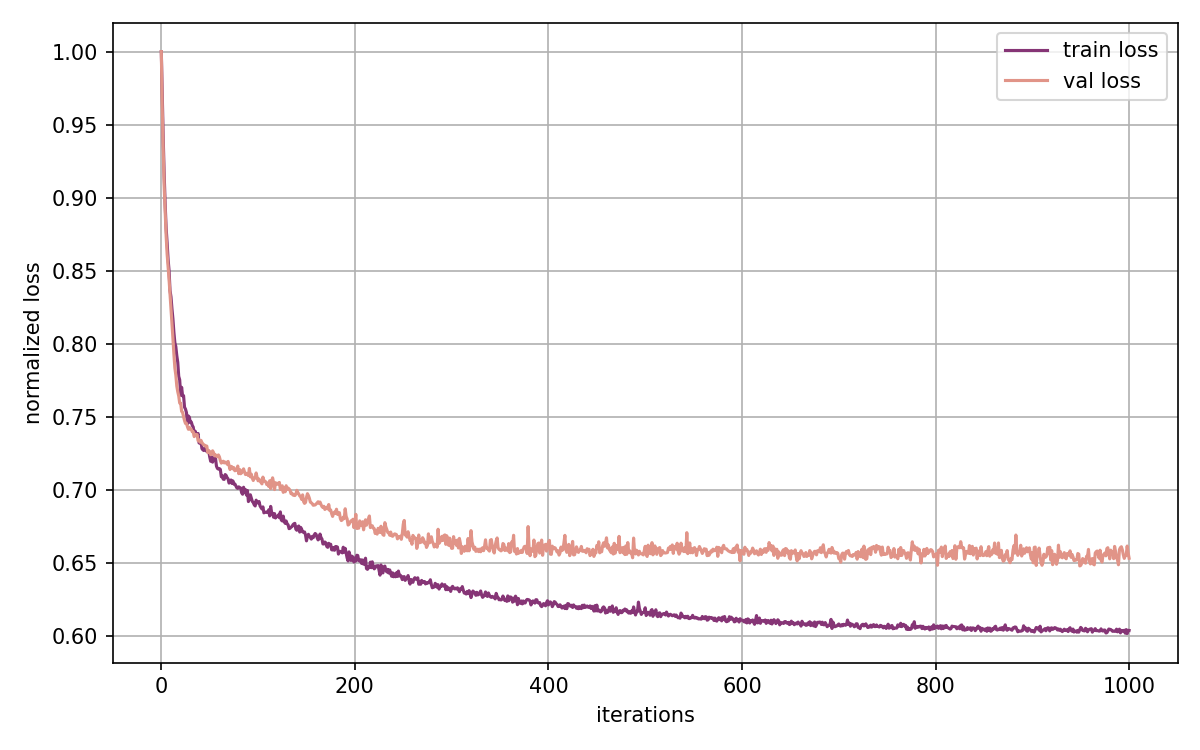
\includegraphics[width=0.45\textwidth]{./4_practice/figs/ml_adv_fc3_train_loss_label}}
    \subfigure[random init]{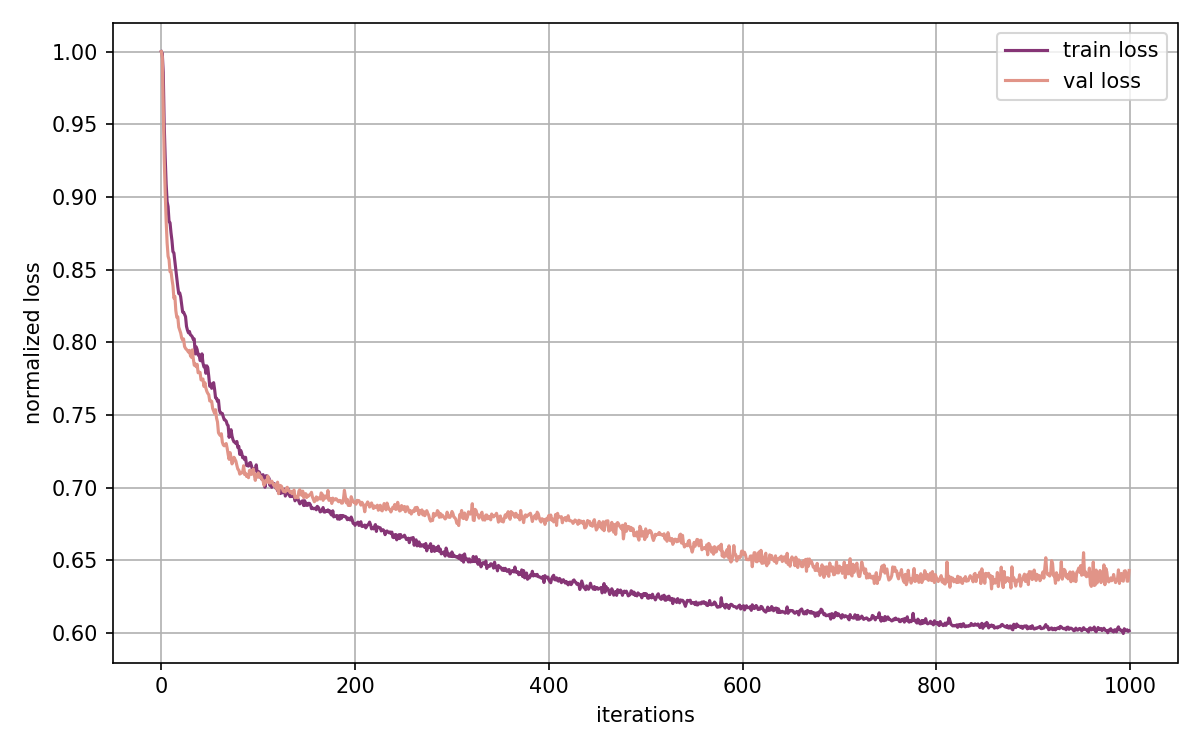
\includegraphics[width=0.45\textwidth]{./4_practice/figs/ml_adv_fc3_train_loss_random}}
  \caption{Comparing the train loss of L5-n500-norm1, c1d0dd0e0-norm1-it1000-bs32-lr0.0001-mo0.5 once with random init and once with adv init with dec-itl1000.}
  \label{fig:ml_adv_fc3_train_loss}
\end{figure}
\FloatBarrier
\noindent

\begin{figure}[!ht]
  \centering
    \subfigure[adv init]{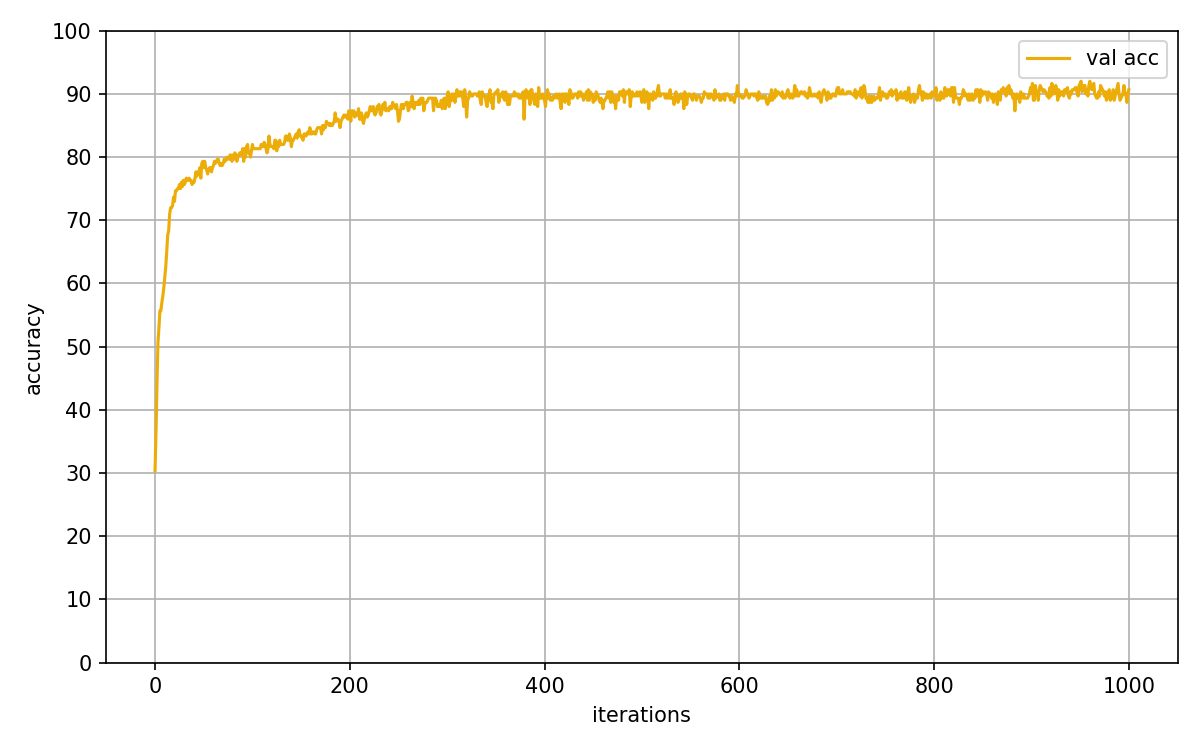
\includegraphics[width=0.45\textwidth]{./4_practice/figs/ml_adv_fc3_val_acc_label}}
    \subfigure[random init]{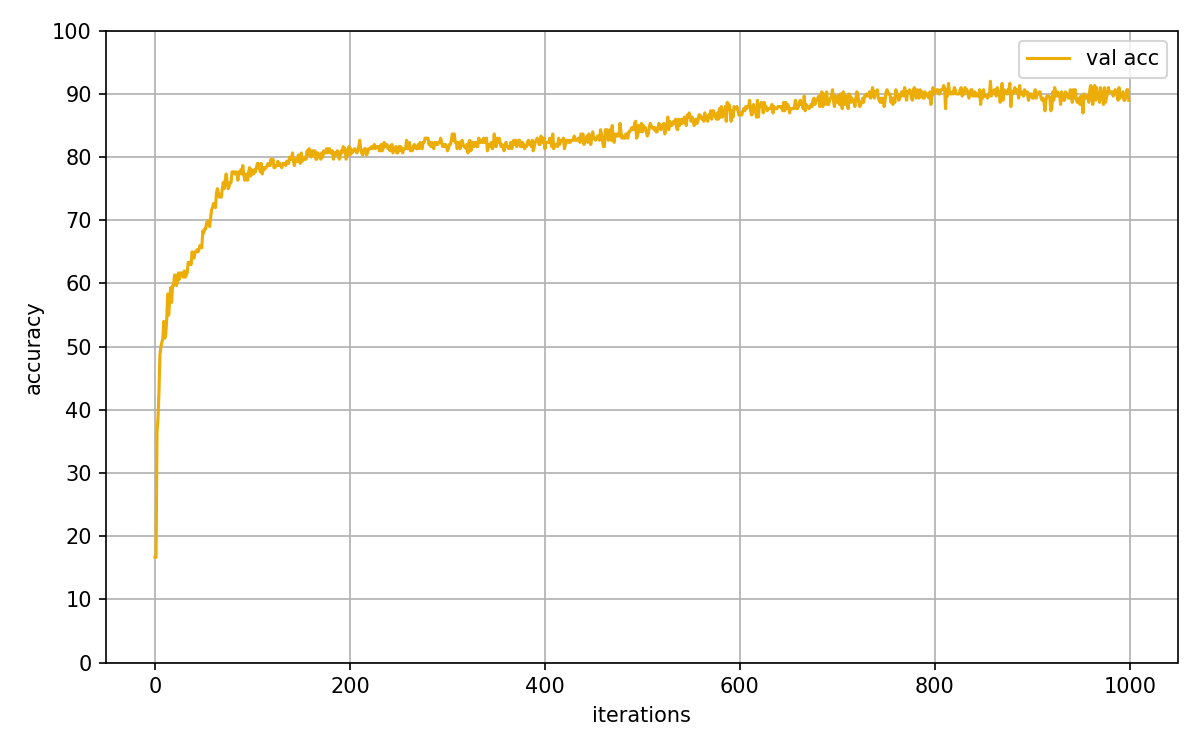
\includegraphics[width=0.45\textwidth]{./4_practice/figs/ml_adv_fc3_val_acc_random}}
  \caption{Comparing the validation accuracy of L5-n500, c1d0dd0e0-norm1-it1000-bs32-lr0.0001-mo0.5 once with random init and once with adv init with dec-itl1000.}
  \label{fig:ml_adv_fc3_val_acc}
\end{figure}
\FloatBarrier
\noindent

The loss and accuracy plots show how well the training was going forward for this showcase example. Both training work well and seem to converge, the one of the adversarial init parameters has a considerably faster convergence time here than the one without.
The scores on the test sets are shown in \rtab{ml_adv_fc3_score}, where both are achieving high scores on the test set, while the adversarial init one got a few percent more, but less on the my set.
This does not necessarily proof if one method is better or worse, therefore a more challenging task must be picked.
But at least it shows that adversarial pre training works at least as good as random initialization.
\begin{table}[ht!]
\begin{center}
\caption{Score comparison on arch: conv-encoder-fc3 with dataset: L5-n500 and training params: c1d0dd0e0-norm1-it1000-bs32-lr0.0001-mo0.5 and different adv params.}
\begin{tabular}{ M{2cm}  M{1.5cm}  M{1.5cm} }
\toprule
\textbf{adv params} & \textbf{acc test} & \textbf{acc my} \\
\midrule
none & 88.33 & 93.33 \\
dec-itl-1000 & 91.67 & 90.00 \\
\bottomrule
\label{tab:ml_adv_fc3_score}
\end{tabular}
\end{center}
\end{table}
\FloatBarrier
\noindent


\subsection{Wavenets}
Wavenets is great...

% game design
\section{Video Games}
video games...



